\documentclass[]{article}

\usepackage{graphicx}
\usepackage{listings}
\usepackage{color}

\graphicspath{ {./images/} }

\definecolor{dkgreen}{rgb}{0,0.6,0}
\definecolor{gray}{rgb}{0.5,0.5,0.5}
\definecolor{mauve}{rgb}{0.58,0,0.82}

\lstset{frame=tb,
	language=Java,
	numbers=left,
	numberstyle=\scriptsize,
	aboveskip=3mm,
	belowskip=3mm,
	showstringspaces=false,
	columns=flexible,
	basicstyle={\small\ttfamily},
	numbers=none,
	numberstyle=\tiny\color{gray},
	keywordstyle=\color{blue},
	commentstyle=\color{dkgreen},
	stringstyle=\color{mauve},
	breaklines=true,
	breakatwhitespace=true
	tabsize=3
}

\lstdefinelanguage{json}{
	basicstyle=\normalfont\ttfamily,
	numberstyle=\scriptsize,
	stepnumber=1,
	numbersep=8pt,
	showstringspaces=false,
	breaklines=true,
	frame=lines,
	literate=
	*{0}{{{\color{mauve}0}}}{1}
	{1}{{{\color{mauve}1}}}{1}
	{2}{{{\color{mauve}2}}}{1}
	{3}{{{\color{mauve}3}}}{1}
	{4}{{{\color{mauve}4}}}{1}
	{5}{{{\color{mauve}5}}}{1}
	{6}{{{\color{mauve}6}}}{1}
	{7}{{{\color{mauve}7}}}{1}
	{8}{{{\color{mauve}8}}}{1}
	{9}{{{\color{mauve}9}}}{1}
	{:}{{{\color{dkgreen}{:}}}}{1}
	{,}{{{\color{dkgreen}{,}}}}{1}
	{\{}{{{\color{delim}{\{}}}}{1}
	{\}}{{{\color{delim}{\}}}}}{1}
	{[}{{{\color{delim}{[}}}}{1}
	{]}{{{\color{delim}{]}}}}{1},
}
%opening
\title{Relazione progetto Reti WORTH}
\author{Fulvio Denza, 544006, f.denza@studenti.unipi.it}

\begin{document}

\maketitle

\section{Introduzione}
WORTH è un modo per condividere il workflow di un progetto. Esso rappresenta una delle metodologie AGILE che si sono sviluppate negli ultimi anni. Il modello di WORTH è un modello semplificato di applicativi del campo, quali easy redmine, trello e molti altri. In WORTH vediamo l'esistenza di una sequenza di stati dei vari task, quale todo, in progress, to be revised e done, la presenza di una chat per ogni progetto, azioni basilari sulle card (o task) quali change status, add card, get card history ed altre.

Il modus operandi per presentare i comandi del progetto sarà bilaterale, ossia verrà descritto l'azione del client e la risposta del server, mentre le strutture dati e le scelte di implementazione delle astrazioni saranno presentate nelle rispettive sezioni del server o del client.

\section{Package Server}
Il server contiene la logica del nostro applicativo, contiene le Classi per descrivere le componenti di WORTH, esso parte da una classe Main.
\subsection{Main}
Il main presenta le istanziazioni delle classi per la connessione TCP e per la RMI Callback
\begin{lstlisting}[language=java]
	//Main.java
	//REGISTER
	UserRegister ur = new UserRegister();
	Runtime.getRuntime().exec("rmiregistry 2020");
	System.setProperty("java.rmi.server.hostname","0.0.0.0");
	ur.RemoteHandler(5455);
	
	//LOGIN
	ServerNotification serverCB = new ServerNotification();
	ServerNotificationInterface stubCB = (ServerNotificationInterface) UnicastRemoteObject.exportObject(serverCB, 0);
	String name = "notification";
	LocateRegistry.createRegistry(7001);
	Registry registryCB = LocateRegistry.getRegistry(7001);
	registryCB.bind(name, stubCB);
	
	//TCP Connection
	TCPConnection connection = new TCPConnection(serverCB);
	connection.start(5456);
	if(Thread.interrupted()) connection.stop();
	System.out.println("Server Started");
\end{lstlisting}
Le righe di codice sopra riportate presentano semplicemente l'istanziazione delle classi Server per le nostre RMI Callback che verranno invocate nel momento in cui il client effettuerà una register e una login. La TCP Connection è il modo in cui viene istanziato il server TCP per aprire il canale di comunicazione lato server implementato per mezzo di una ServerSocket sulla porta 5456.\\
\begin{center}
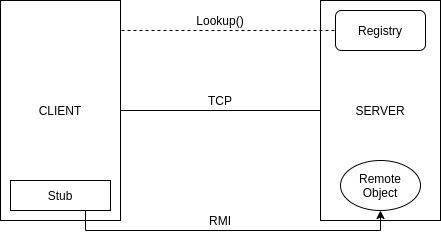
\includegraphics[scale=0.6]{classDiagram}
\end{center}
\subsection{Database}
Il database è stato sviluppato usando la libreria di Google gson, esso consiste in un file .json contenente tutti gli utenti nella forma:
\begin{lstlisting}[language=json]
	n:
		username: "username"
		password: "password"
		projectList:
			0: "project"
			1: "project"
			...
\end{lstlisting}
in cui n è l'indice, nel file json, della posizione dell'utente, il campo username e password sono i campi in cui vengono conservati le relative informazioni, projectList contiene, invece, la lista di progetti a cui appartiene l'n-esimo utente.
Una miglioria, nonchè best practice, sarebbe potuta essere implementare un algoritmo di crittografia per salvare le password cifrate, anzichè in chiaro, tuttavia ai fini del progetto non era strettamente necessario.
\section{Package Client}
\end{document}
